This chapter tackles \ref{rq:4} by analyzing how \acp{DTE} and \ac{MAS} can be used synergistically to engineer intelligent IoT systems and applications.
%
Since both abstractions have been used to encapsulate intelligence in IoT systems, it is crucial to clarify their respective roles and responsibilities to avoid confusion and overlapping solutions.
%
This has been partially explored in the literature before (\Cref{sec:back:mas:dt+mas}) but not yet systematically addressed from a software engineering perspective.

This chapter aims to fill this gap by providing a comprehensive analysis of the synergies between \acp{DT} and \ac{MAS}.
%
The resulting proposal is grounded in a set of design principles that help system designers decide when to use \acp{DT}, when to use \acp{MAS}, and how to combine them effectively.

%=======================================================
\section{Complementarity of DTs and MAS}
%=======================================================

Autonomous Agents (AAs) and Digital Twins (DTs) are gaining increasing attention in the literature about the distribution of intelligence in IoT systems and applications (\Cref{sec:back:mas:dt+mas}). 
AAs encapsulate reasoning routines and decision-making criteria tailored to a given goal. 
Hence, they naturally lend themselves to implement the perception-action feedback loop typically required in the IoT to realize the ``actionable knowledge'' paradigm~\cite{Barnaghi2013}. 
DTs digitalize an entity of interest in the physical world to decouple applications and services from the technical intricacies of interacting with such entities. 
Also, they may offer additional digital functions (i.e. \emph{augmenting} the behavior of physical entities~\cite{dt-IoT-context-Minerva-2020}). 
Thus, they both naturally fit the IoT context in bridging together the ``cyber'' and the ``physical'' parts of a system.
%
Consequently, to date, several approaches and architectures have been proposed employing either one abstraction or the other, or even both combined~\cite{Mariani_Picone_Ricci_2022,Kalyani_Collier_2024,Pretel_Moya_Navarro_López-Jaquero_González_2024}, to enable \emph{distributed intelligence}~\cite{Rosendo_Costan_Valduriez_Antoniu_2022,Alsboui_Qin_Hill_Al-Aqrabi_2021}. 

However, it is not always clear what the \emph{relationship} between these abstractions is at both the architectural and technological level: namely, whether AAs and DTs are interchangeable, (partially) overlapping, alternatives, complementary, or anything else. 
%
In those works that propose an integration, it happens in many different ad-hoc ways: for instance, with ``multi-agent based DTs'' to digitalize complex systems of the real world~\cite{Pretel_Zhinin-Vera_Navarro_López-Jaquero_González_2025}, or with AAs using DTs as a digital substrate to deal with interoperability~\cite{web-of-dt-ricci-2022}. 
%
As a consequence, there is an emerging \emph{fragmentation}: the existence and proliferation of several solutions to the same problems, which have no clear relationships with each other, and that are conceived for specific applications. 

In fact, as most of these approaches are proposed in the context of a specific application or intended goal, there is little interest in providing IoT systems and application engineers with general principles to guide their design choices regardless of the specific application domain and/or goal. 
%
Arguably, that this lack of clarity is problematic for the broader IoT community, as it leads to a variety of approaches that may tackle similar problems with different solutions, keeping closed vertical silos between partially overlapping communities.

This section briefly reports exemplary works that discuss the application of either AAs or DTs in \ac{IoT} systems, highlighting their respective contributions to the design of intelligent functionalities.
%
This effort goes towards highlighting the complementary roles of these abstractions in engineering intelligent IoT systems, paving the way for defining design principles to guide the separation of concerns between the two abstractions. 

%-----------------------------------------------------
\subsection{Use of AAs and DTs in IoT Systems}
%-----------------------------------------------------

Agents and MAS have been widely used in many domains primarily as a context-aware model and technology to encapsulate intelligent behavior in \emph{distributed} and \emph{reusable} software components (\Cref{chap:back:MAS})
%
This includes the IoT domain, 
that is a good fit for agents' situated decision-making abilities~\cite{Savaglio2020}: sensors and actuators provide the means to perceive and affect the real world (a physical environment), while agents encapsulate the system's \emph{goals} and the reasoning processes needed to bring the system in the desired state of affairs---by closing the feedback loop between sensing and acting.
%
From a distributed system perspective, MAS improves IoT by addressing autonomy and heterogeneity, enabling device and data discovery through semantic service descriptions, fostering trust through reputation and incentives, and facilitating collective intelligence~\cite{Singh_Chopra_2017}. 

\Cref{tab:aa_technology_papers} summarizes a selection of representative works that exploit AAs in IoT systems to deliver different intelligent functionalities.

\begin{table}
    \centering
    \renewcommand{\arraystretch}{1.2}
    %\setlength{\tabcolsep}{8pt}
    \footnotesize
    \begin{tabularx}{\textwidth}{|p{2.75cm}|p{2.75cm}|X|}
        \hline
        \textbf{Intelligent Functionality} & \textbf{Representative Papers} & \textbf{Notes} \\
        \hline
        \emph{Logic inference} & \cite{Omicini_Calegari_2019} \cite{longo-2021} \cite{DBLP:journals/pieee/LeitaoKRLSC16} \cite{DBLP:journals/jms/CicirelliFGGSV16} & Works applying logic-based approaches in IoT systems to improve explainability and deductive reasoning of the system components. \\%Historically the premier application of AAs in AI, as symbolic reasoning in general. \\
        \hline
        \emph{Adaptive control} & \cite{Savaglio_Fortino_Zhou_2016} \cite{lanza-2020} \cite{Ciortea_Mayer_Michahelles_2018} \cite{DBLP:journals/pieee/LeitaoKRLSC16} \cite{DBLP:journals/tii/ZhangQLL17} \cite{DBLP:journals/access/TangLWD18} & Works showcasing the effectiveness of adaptive behavior of agents in IoT settings, highlighting properties such as context- and self-awareness as well as planning for dynamic reconfiguration. \\ %Another typical application of AAs for encapsulating control policies and decision-making depends on contextual information. \\
        \hline
        \emph{Learning of control policies} & \cite{rosenberger-2022} \cite{yang-2021} \cite{DBLP:journals/comsur/LeiTZLZS20} \cite{DBLP:journals/rcim/ZhouTZZ21} \cite{DBLP:conf/itsc/LiuLC17} \cite{DBLP:journals/tvt/ZhangMZXSH23} & Works showcasing applied scenarios of Multi-Agent Reinforcement Learning and Deep Reinforcement Learning to learn cooperation policies. \\%A more recent trend arose with the success of reinforcement learning techniques, where AAs are not programmed, but learn how to do something. \\
        \hline
        \emph{Simulation} & \cite{laghari-2016} \cite{butt-2020} \cite{DBLP:journals/pieee/LeitaoKRLSC16} & Works describing simulations of IoT scenarios performed with a multi-agent based model to simulate the interactions between autonomous components.\\%Another traditional application domain for AAs, although often, and especially in MABS, the agent notion is quite weak. \\
        \hline
    \end{tabularx}
    \caption{Selection of literature on AAs exploitation in IoT for delivering different intelligent functionalities.}
    \label{tab:aa_technology_papers}
\end{table}


% %-------------------------------------------------------------
% \subsection{Use of Digital Twins Encapsulating Intelligence}
% %-------------------------------------------------------------

Similarly to AAs , \acp{DT} are increasingly used to encapsulate intelligent functionalities that enhance the capabilities of the \acp{PA} they digitalize.

The relationship between \acp{DT} and intelligence in IoT systems has been widely explored in the literature (\Cref{sec:back:dt:ai}).
%
\Cref{tab:dt_technology_papers} summarizes a selection of representative works that exploit \acp{DT} in IoT systems to deliver different intelligent functionalities.
%
\acp{DT} can leverage data collected from their corresponding \acp{PA} to perform various intelligent tasks.
%
The modeling capabilities that are intrinsic to \acp{DT} is often associated with simulation, forecasting and anomaly detection functionalities.


\begin{table}
    \centering
    \renewcommand{\arraystretch}{1.2}
    %\setlength{\tabcolsep}{8pt}
    \footnotesize
    \begin{tabularx}{\textwidth}{|p{2.75cm}|p{2.75cm}|X|}
        \hline
        \textbf{Intelligent Functionality} & \textbf{Representative Papers} & \textbf{Notes} \\
        \hline
        \emph{Prediction and Learning} & \cite{Elayan_Aloqaily_Guizani_2021} \cite{Hu2022} \cite{Qiao2019} \cite{Qian2023} \cite{DBLP:journals/tvt/ZhangWXZLNH23} \cite{DBLP:journals/tifs/AliKLYTP23} \cite{MULLER2022126} & Prediction of future states of a PA is one of the most common intelligent functionalities delivered by DTs, together with simulation (see below). Such predictions are increasingly delivered via data-driven, machine learning techniques. \\
        \hline
        \emph{Inference} & \cite{DBLP:journals/access/XuSLZ19} \cite{dt_automated_behavior_analysis} \cite{QIAN2024111349} \cite{DBLP:journals/iotj/ZhouLQ24} & DTs are also used to synthesize novel information either based on historical data gathered about the PA, or by aggregating the data of multiple PAs that are so tightly coupled in the physical world to be worth digitalizing them altogether with a single DT. \\
        \hline
        \emph{Simulation} & \cite{Boschert_Rosen_2016} \cite{Hofmann2019} \cite{Elahi2021} \cite{Karakra2019} \cite{Danilczyk_Sun_He_2019} \cite{DBLP:journals/jsac/WangDWRGD23} \cite{QIAN2024111349} & Simulation of alternate configurations or working conditions for a given PA is another typical application of DTs. \\
        \hline
    \end{tabularx}
    \caption{Selection of literature on DTs exploitation in IoT for delivering different intelligent functionalities.}
    \label{tab:dt_technology_papers}
\end{table}


%-------------------------------------------------------------
\subsection{Intelligent Functionalities}
\label{ssec:mas+dt:functionalities}
%-------------------------------------------------------------


The literature on distributing intelligence in IoT reports on several intelligent functionalities for which AA and DTs are being actively used by system designers. 
%
Here they are summarized focussing on the \textit{kind} of intelligent function they deliver, regardless of the specific task they accomplish (e.g.\ time series forecasting vs.\ fault prediction) and of the specific technique adopted (e.g.\ regression, SVM, etc.).
%
This categorization is useful in defining what can be considered, ``intelligence'' in a practical, bottom-up way, stemming from related works in the area without getting trapped in philosophical arguments.
%
Then, it is also useful to establish the \emph{coverage} of such functionalities by AAs and DTs as emerging from \Cref{tab:aa_technology_papers} and \Cref{tab:dt_technology_papers}.

\begin{description}
    \item[\emph{Prediction}] there including time series forecasting, recommendations, namely any form of reasoning meant to ``guess'' new information based on past and current knowledge. 
    In the IoT, common prediction targets are machinery failures, stock levels, resource use, and system states.


    \item[\emph{Simulation}] encompassing any form of hypothesizing different states, in the past, present, or future. 
    ``What-if''-like analysis falls into this category. 
    In the IoT, it is common to simulate the future states of individual things, for example, to improve the design of a product or a production pipeline. 
    However, complete systems can also be simulated with an added degree of complexity.


    \item[\emph{Planning}] that includes any form of synthesis, and \emph{practical reasoning}~\cite{Bratman1987-BRAIPA}, which is meant to figure out how to achieve some practical effect (on the target system) by properly sequencing available actions. 
    Planning to achieve a given system configuration is common in the IoT, as well as planning to reconfigure after some disruptions. 


    \item[\emph{Inference}] within which both \emph{epistemic reasoning}~\cite{Meyer1995}, that is, synthesizing novel information from known data, or data-driven inference such as pattern recognition and classification.
    This is perhaps the most common form of intelligence used in IoT, as even simple monitoring and control applications usually infer situations by aggregating different data coming from distributed sources of information. 
    In addition, fault detection and diagnosis can be gathered in this category. 


    \item[\emph{Adaptation}] instead gathers all the intelligent functionalities aimed at enabling the system to adapt to unforeseen situations that had not been explicitly managed at design time. 
    As in the previous category, this one is quite broad and includes several heterogeneous approaches, ranging from engineered adaptation (e.g.\ the MAPE-K loop~\cite{Kephart_Chess_2003}) to learning-based methods (e.g.\ evolutionary approaches~\cite{Eiben2005}). 


    \item[\emph{Learning}] which despite not usually being the primary goal for a functionality, is a valuable tool to implement some of the ones highlighted above and still poses important requirements on the architecture of a system that wishes to support any form of learning process in one of its components.
    That includes statistical machine learning, reinforcement learning, and causal structure learning. 
    This category groups functionalities that aim to make the system, or one of its components, learn to do something. 
    In IoT, the most common form of learning employs statistical machine learning to create prediction models, for example. 


\end{description}

These high-level categories of intelligent functionalities will guide the analysis of how to distribute them across AAs and DTs in the rest of this chapter.

%=======================================================
\section{Design Principles}
%=======================================================

In an attempt to clarify the complementary roles of \acp{DT} and \ac{MAS} in engineering intelligent \ac{IoT} systems, a set of design principles are proposed in this section, to guide the analysis from a functional standpoint, i.e.\ focusing on the intelligent functionalities to be delivered by the system.
%
The proposed principles can then be used to inform the design of architectural patterns that combine \acp{DT} and \ac{MAS} effectively. 

The principles are derived from the quite abstract software engineering criterion of \emph{separation of concerns} given in~\cite{Mariani_Picone_Ricci_2022}, expanding and refining it along three dimensions to make it more practically useful: \emph{specificity}, \emph{scope}, and \emph{time}. 
%
These are meant to be used to analyze the requirements posed by the intelligent functionalities identified in the previous section. 

Neither of these dimensions \emph{alone} is sufficient to determine \emph{univocally} which abstraction is best suited for a given functionality. 
Instead, they all need to be taken into consideration together when approaching the design of an intelligent IoT system as shown in \Cref{sec:mas:mas+dt:example}.


%--------------------------------------
\subsection{Specificity} 
%--------------------------------------

The first proposed principle is named \emph{specificity}, whose spectrum is depicted in \Cref{fig:specificity}, and is defined informally as 
\begin{quote}
    ``how much a given (intelligent) functionality is \emph{specifically} serving a given application goal (at one end of a spectrum), rather than being \emph{generally} exploitable by multiple goals and potentially across application scenarios (at the other end)''.
\end{quote}
%
This aims to help IoT systems and application designers to distinguish between
\begin{itemize}
    \item features that are strictly tied to the achievement of a specific \emph{application goal}
    \item features that may be \emph{generically} useful to pursue multiple goals and build other intelligent functionalities and/or applications on top.
\end{itemize}
%
This is especially important for designing highly modular systems that can evolve over time.

\begin{figure}
    \centering
    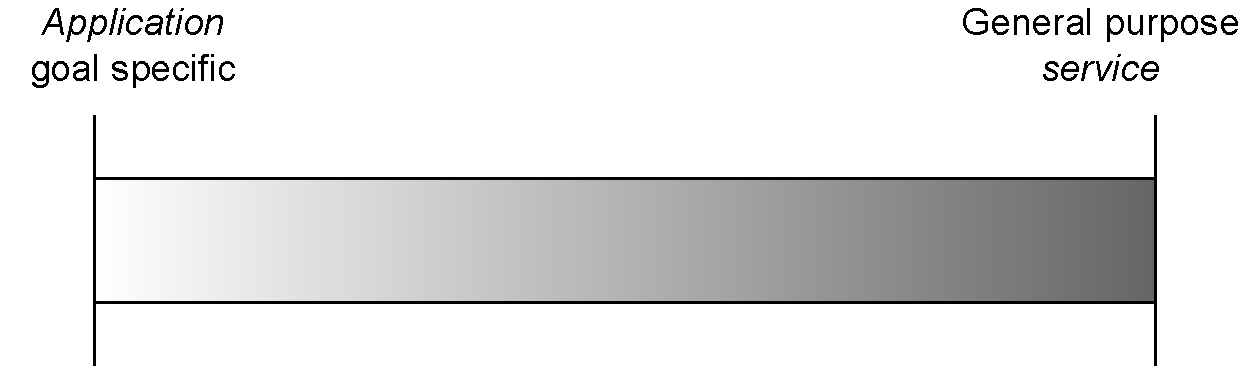
\includegraphics[width=.6\columnwidth]{figures/dt-mas/specificity-spectrum.pdf}
    \caption{The spectrum of \emph{specificity}: from intelligent functionalities specific to an application goal to general-purpose services.}
    \label{fig:specificity}
\end{figure}

In IoT systems, for instance, a widespread general-purpose functionality concerns the digitalization of \acp{PA} to enable intelligent functionalities such as prediction of that assets' future states, and simulation of alternate states. 
%
Functionalities like these can be considered to be not tied to the application goals, but to the general services offered by the IoT platform, in an open-system, ``as-a-service'' perspective.

In contrast, functionalities such as fault diagnosis or inference of specific information may be relevant only in the context of the application domain or goal. 
Another example would be the implementation of adaptive control policies and decision-making strategies: these are likely to be specialized for the system at hand, as they encode the requirements and goals set by stakeholders. 

For instance, in a smart building, there could be several control policies introduced to optimize comfort or energy consumption.
%
Those policies will be part of the system due to a specific requirement coming from the stakeholders.
%
At the same time, the building may also include functionalities that are more general-purpose, such as predicting the future energy consumption of the building based on historical data.
%
This may serve multiple goals, such as optimizing energy use, improving occupant comfort, or reducing operational costs.

%-----------------------------------------
\subsection{Scoping} 
%-----------------------------------------

The second proposed principle, is named \emph{scoping}, and is defined as follows:
\begin{quote}
    ``to what extent a given (intelligent) functionality requires data from the whole system (at one end of a spectrum) or a single individual entity of interest (at the other end) to deliver its results''
\end{quote}
This aims to help IoT systems and applications designers distinguish between:
\begin{itemize}
    \item features that require data, inputs, and interactions with multiple entities of interest in the system at hand (up to \emph{global} information, synthesized at the system level);
    \item features that require only considering a single asset (the extreme case of \emph{local} information).
\end{itemize}
Figure~\ref{fig:scope} depicts this spectrum. 

\begin{figure}
    \centering
    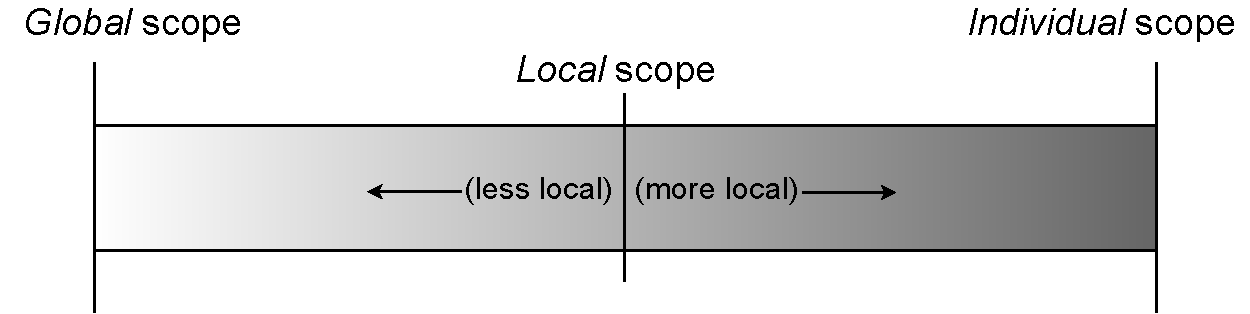
\includegraphics[width=.6\columnwidth]{figures/dt-mas/scope-spectrum.pdf}
    \caption{The spectrum of \emph{scoping}: from intelligent functionalities requiring knowledge of the whole system, to those confined to individual assets.}
    \label{fig:scope}
    
\end{figure}


In any IoT system, due to its inherent connection with the physical world, there are software components whose main function 
is to digitalize individual, clearly identifiable domain entities or a specific portion of the physical world. 
Such software components 
are coupled with PAs, which set boundaries to the \emph{scope} within which intelligent functionalities operate. 

For example, a component might be designed to collect and train on local information only (e.g.\ prediction of the future states of specific machinery, not others). 
%
Conversely, many other functionalities may require a broader scope that goes well beyond such local boundaries. 
For instance in the domain of a smart home,
software components may mirror, and grant access to, the individual devices (e.g.\ for remote monitoring and control), 
but there could also be adaptive control routines spanning multiple devices or even multiple rooms to orchestrate a coordinated action (e.g.\ preparing for the comeback of an inhabitant by activating the A/C, unlocking the doors, raising the curtains, etc.). 
%
Accordingly, the scoping principle is meant to suggest that system designers consider where the knowledge and data required to accomplish the intelligent function come from, as well as which entities will be subject to its effects. 

It should be noted that the \emph{individual} and \emph{global} scopes are the two extremes of the spectrum depicted in Figure~\ref{fig:scope}. 
Functionalities may require data from multiple entities, but such entities may be confined in a limited space, for instance geographically, or network-wise. 
Or, it could be the case that data is required from different and distant entities that are anyway somehow easy to access together---think of overlay networks. 
%
In this case, the proposed principle is still useful to guide design choices, as it forces designers to clarify and sort out why and how they deem the scope to be worth defining global or local (or even individual). 

%--------------------------------------
\subsection{Timing} 
%--------------------------------------

The third (and last, for the time being) proposed principle is what named \emph{timing}, and defined informally as 
\begin{quote}
    ``how much a given functionality relies on any one notion of \emph{time} (e.g.\ physical or logical) to be either explicitly (i.e.\ \emph{time-aware}) or implicitly (i.e.\ \emph{time-situated}) available''
\end{quote}
%
The concept of ``time-aware'', is meant to convey that the functionality requires access to time-related information, either to make it directly observable to consumers of such functionality or to work properly. 
For instance, time series forecasting (a form of prediction) needs an explicit representation of time to be available, hence it is time-aware. 

The concept of ``time-situated'', instead, conveys that the functionality has some dependency on any one notion of time, but such dependency need not be explicitly captured and managed. 
For instance, real-time monitoring and control of an asset surely depend on time, but such a dependency need not be modelled explicitly to deliver the functionality. 
%
Simply, its existence suffices for the functionality to work properly.
There are also some other cases where time does not matter from the designer's standpoint, as time is not an issue when implementing the functionality---e.g., sending commands to an actuator device. 
This whole spectrum is depicted in \Cref{fig:timing}. 

\begin{figure}
    \centering
    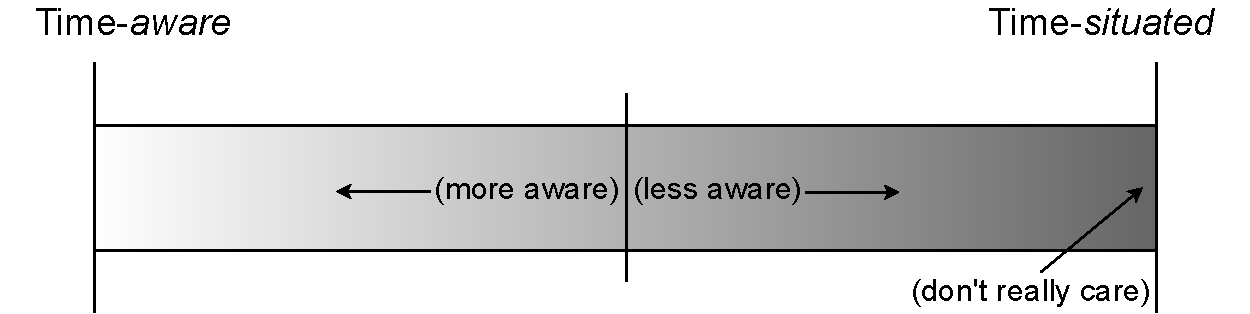
\includegraphics[width=.6\columnwidth]{figures/dt-mas/timing-spectrum.pdf}
    \caption{The spectrum of \emph{timing}: from intelligent functionalities requiring explicit modelling of physical or logical time, to those that don't care.}
    \label{fig:timing}
\end{figure}

Of course, placing intelligent functionalities within this spectrum cannot be a precise operation, as with the other principles. 
But some general considerations about the categories of intelligent functionalities can and should be made to aid system designers. 
%
For example, prediction, simulation, and diagnosis are likely to require time awareness. 
How far into the future should an event or state of interest be predicted? 
How long into the future should a simulation extend? 
Conversely, when did a chain of faults lead to the present faulty situation? 
%
Other functionalities, such as inference, learning, and adaptation, may be less demanding and simply be time-situated. 
Of course adaptation actions are based on some events that happened, or on some predicted future state, and need to be carried out in the future, but possibly they do not require an explicit representation of time to work properly as simply their sequential ordering is sufficient to eventually react accordingly. 

%=======================================================
\section{Matching AAs and DTs to Design Principles}
%=======================================================

The design principles introduced in the previous section are here matched against AAs and DTs, to conceptually assess which abstraction is best suited for which end of the spectrum described above for a given principle. 
Figure~\ref{fig:principles} shows the exemplary functionalities and how they are better encapsulated by AAs or DTs according to the principles. 

\begin{figure}
    \centering
    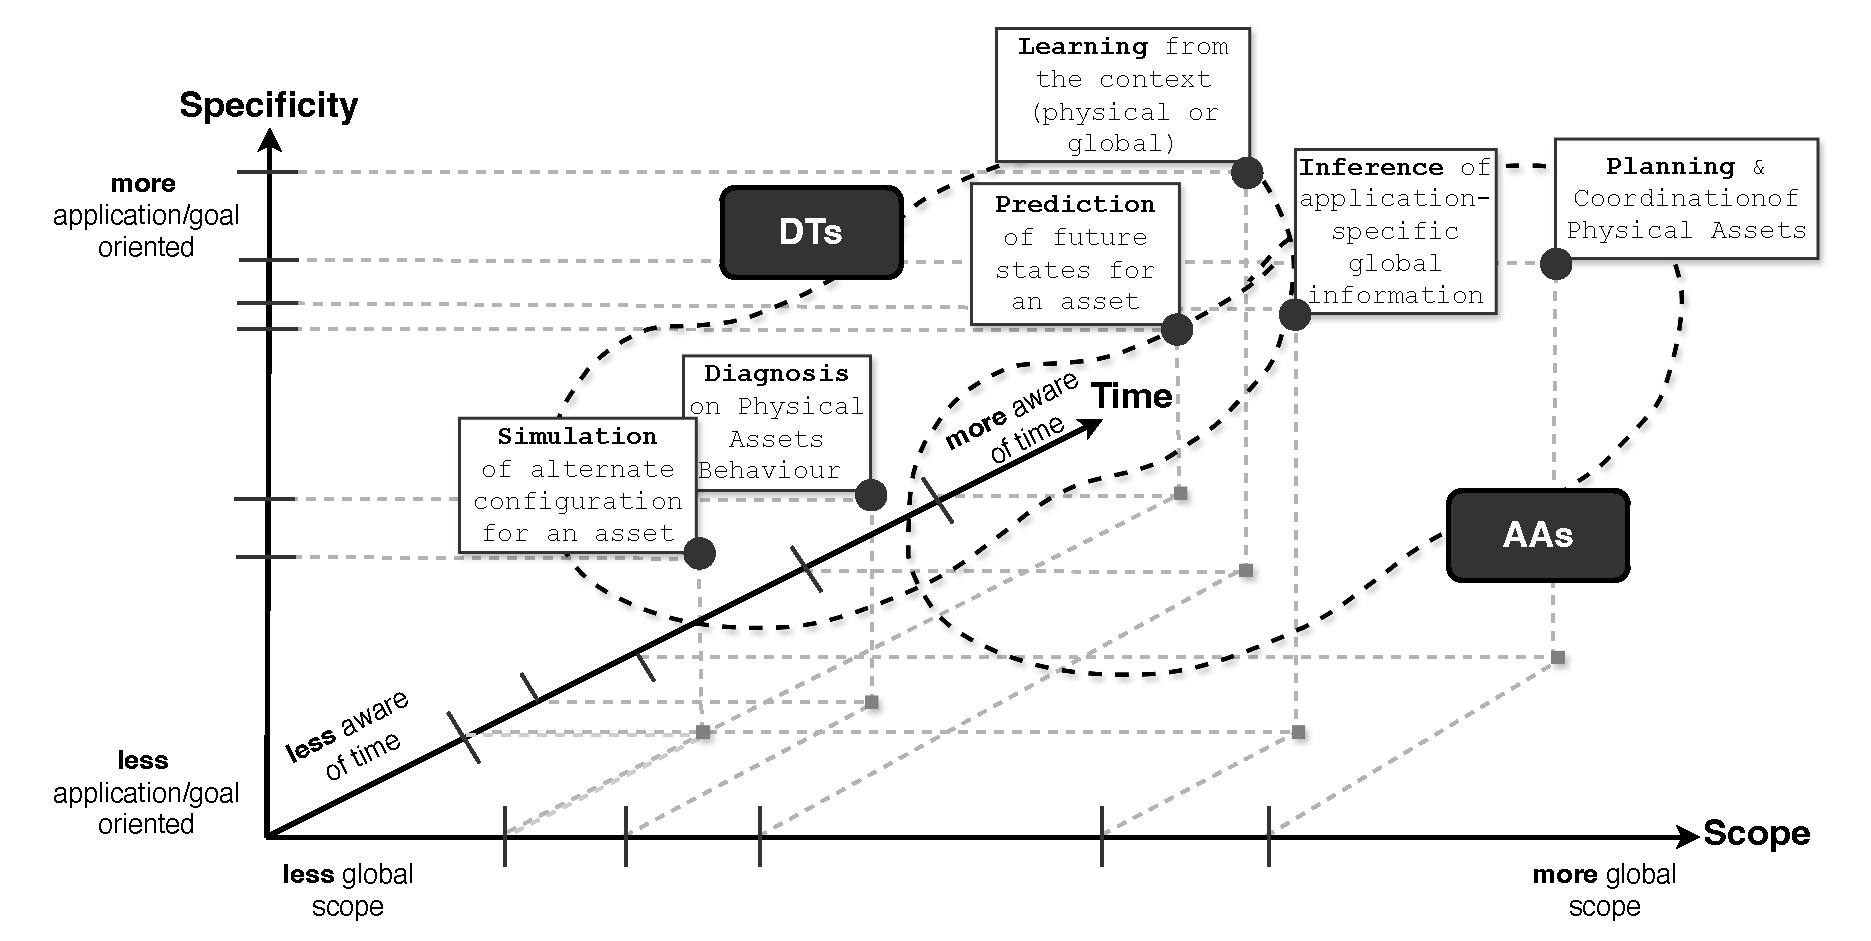
\includegraphics[width=\columnwidth]{figures/dt-mas/principles-aa-dt.pdf}
    \caption{Exemplary intelligent functionalities placed within the spectrum of the proposed design principles. AAs and DTs are clustering those functionalities that they better match with, according to such principles.}
    \label{fig:principles}
\end{figure}

Considering the \emph{specificity} design principle:
\begin{itemize}
\item \textbf{AAs}, being by definition \emph{goal-driven} entities, are usually exploited to encapsulate intelligent functionalities that are strictly related to the problem to solve, hence to the domain and objectives of the application. 
\item \textbf{DTs}, instead, are usually exploited with the scope of digitalising assets to provide data-oriented services to consumer applications, \emph{servitisation} being one of their core characteristics. 
\end{itemize}
The principle of specificity, thus, would encourage designers to encapsulate intelligent functionalities closely matching application goals in AAs, and, complementarily, to model general-purpose services as DTs instead. 

Considering the \emph{scoping} design principle:
\begin{itemize}
\item \textbf{AAs} are not tied to any particular source of information in achieving their goals. 
Although part of the definition of AA includes a relationship with the notion of an environment in which AAs are \emph{situated}~\cite{wooldridge1995ker}, AAs are not limited in any particular way to any given ``object'' in such an environment. 
In other words, the application environment (physical or digital) in its entirety is a source of information that AAs can perceive and (possibly) affect---their \emph{global} scope. 

\item \textbf{DTs}, instead, are specifically defined as being \emph{coupled} with the individual asset in the physical world that they are digitally representing (their physical twin). 
It is thus natural to give DTs a \emph{local} scope, limited to the information available from this physical asset. 
\end{itemize}
Note that the term ``scoping'' is deliberately chosen instead of, for instance, ``locality'', to avoid the misunderstanding that such design principle is inherently tied with some notion of space, such as in a geographical sense or limited by a physical size boundary under which something can be considered local or not.

Scoping simply means that there should be a clear boundary in terms of how many physical assets are involved with the intelligent functionality that designers are considering. 
If an individual asset is the source of information for that functionality, it could be suited to be encapsulated by a DT. 
Otherwise, if the information needed belongs to multiple sources, an AA might be more conceptually aligned.
%
However, the boundary of an individual asset can extend to be a rather large entity.
%
In a smart home, for instance, an asset can be an individual device, a room, or the whole house even. 
Also, nothing prevents an asset from being a composition of multiple others that have a smaller local boundary. 

Finally, with respect to the \emph{timing} principle:
\begin{itemize}
\item \textbf{AAs} do not include any explicit notion of time in their definition. 
    The situatedness feature already mentioned includes the temporal dimension but does not prescribe agents to capture and model time-related aspects. 
    Hence AAs are \emph{time-situated} entities, naturally. 
\item \textbf{DTs}, complementarily, are specifically requested to keep in sync %(shadow)
    their related PA to provide an updated digital representation in a timely manner. 
    This implies explicitly capturing the time at which events in the PA happened, and modelling the temporal evolution of the PAs. %---such as in threading. 
    DTs are thus naturally \emph{time-aware}. 
\end{itemize}

Summarizing the above considerations, AAs and DTs can be described as playing the following roles in the design of distributed intelligent functionalities in IoT systems and applications:
\begin{itemize}
    \item \textbf{AAs} are the components of the IoT system that encapsulate the system/application \textbf{goals}, hence are aware of such specific goals and strive to achieve them by autonomously deciding \textbf{whose other entity} to interact in the whole application domain. 
    AAs are also not particularly tied to any specific notion of time. 
    \item \textbf{DTs}, instead, model and encapsulate properties, behaviors, and functions of specific portions of the IoT system or application domain, therefore are \textbf{inherently bound to specific assets}, to provide \textbf{general-purpose services} to other components or directly to the application. 
    Due to such modelling, DTs must at least account for the specific \textbf{notion of time} relevant to the modelled asset. 
\end{itemize}

%
These definitions are not meant to set crisp boundaries amongst AAs and DTs in any possible use case and scenario. 
%
Consequently, there is a degree of flexibility in how these definitions can be interpreted to distribute responsibilities across different components.
%
However, having well-defined criteria that dictate how to exploit AAs and DTs as complementary abstractions helps to identify responsibilities in the design of an IoT system willing to fully leverage distributed intelligence.

%======================================================
\section{Architectural Integration Patterns}
\label{sec:mas+dt:patterns}
%======================================================

The proposed design principles and their match against AAs and DTs help decide whether an AA or a DT is best suited for a given intelligent functionality. 
However, they tell little about how to combine AAs and DTs \emph{synergistically} when intelligent functionality requires it. 
For instance, because it is positioned within the spectrum of each principle in a way that does not perfectly match all the features of either an AA or a DT, but some of both. 
Accordingly, this section discusses the several ``micro-architectures''  for AAs and DTs integration that may arise during the application of our principles.

The term micro-architecture ($\mu$-arch, for short)  is used to differentiate from the classic \emph{top-down}, ``macro-architecture'' perspective adopted in many \ac{IoT} architectural proposals: what is proposed is a reference architecture for a whole system, a blueprint to adopt in any given IoT scenario (and beyond).
%
% For instance, in the field of enterprise systems architecture, the rise of IoT and the relevance of CPSs in general as the ``backbone'' of many intelligent functionalities within the company (that require asset monitoring and control first and foremost), nurtured research in new designs and methodologies supporting IoT-related goals. 
% There, the general trend is to adopt a \emph{System of Systems} (SoS) perspective over the whole enterprise, decomposing the requirements along the same application-agnostic dimensions. 
% The FCBPSS architecture is an example \cite{DBLP:journals/eis/WangWDFKIZ16}, where the many systems supporting operations of an enterprise are seen in terms of Functions, Context, Behaviour, Principles (guiding the design), Structure (components realising the function and their relations), and State. 
% These very same concepts are applied recursively for the whole enterprise integration system---indeed, a SoS.
%
In contrast, this work follows a bottom-up approach, where the architecture of the overall system is the result of the composition of multiple $\mu$-arch, depicted in\Cref{fig:architecture} by making use of the following components: 
\begin{inlinelist}
\item 
Physical Assets (``PA'' squares), which represent the entities in the real world (e.g. devices, objects, people, processes, organizations) that the IoT system needs to model; 
\item 
DTs (``DT'' circles); 
\item 
AAs (``A'' circles); 
\item 
and the intelligent functionalities (the 3D boxes), which may be entire applications or simply one of the many functions needed for the application at hand. 
\end{inlinelist}


\begin{figure}
    \centering
    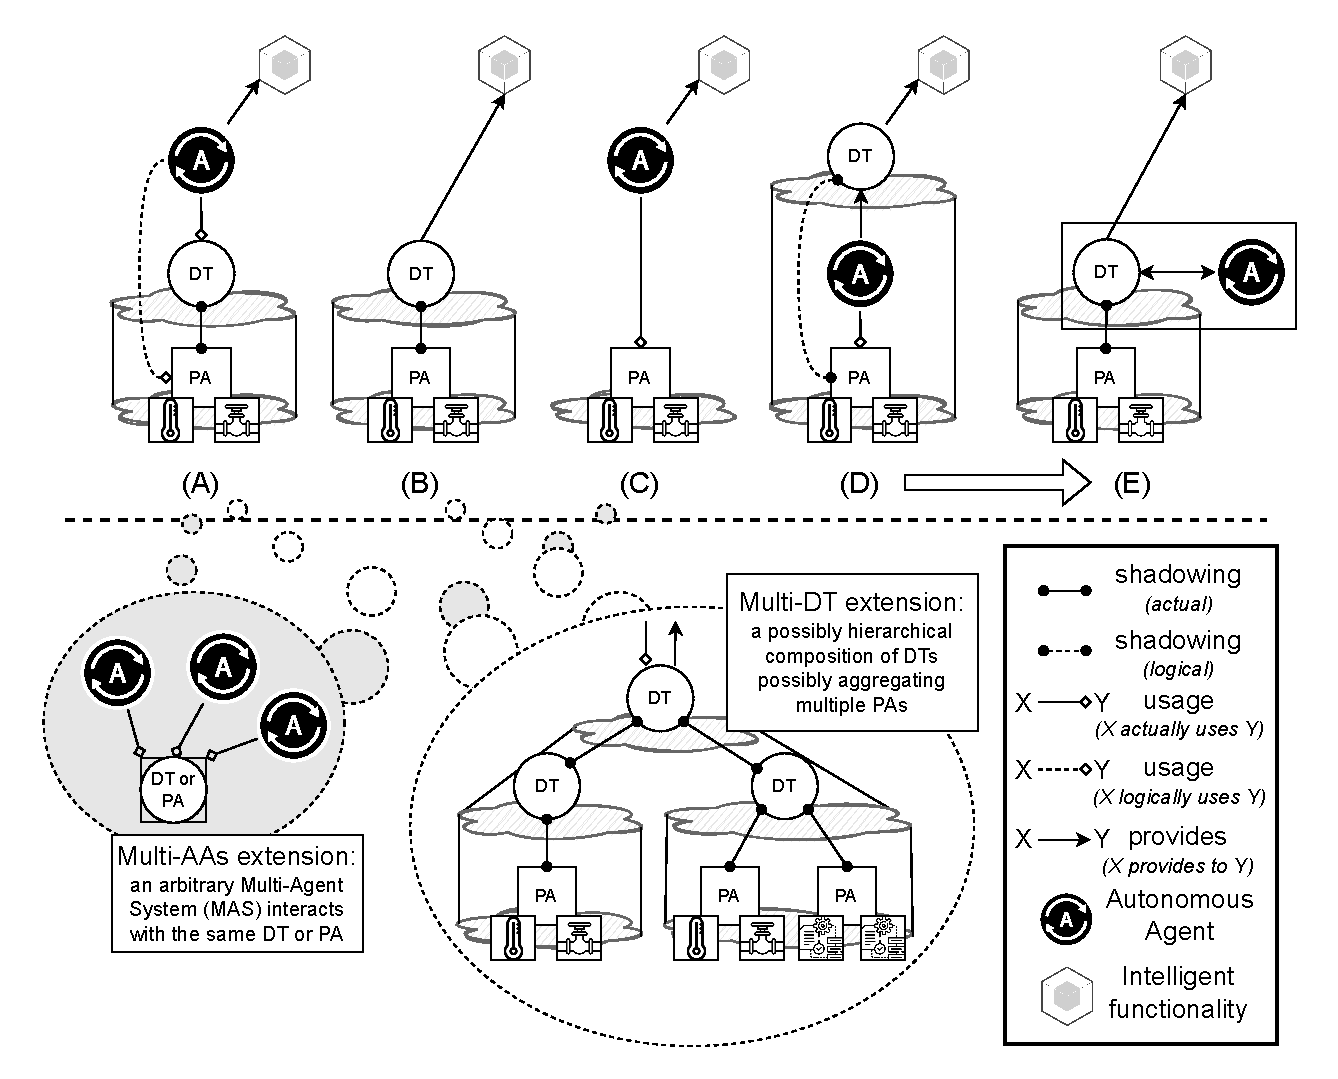
\includegraphics[width=\columnwidth]{figures/dt-mas/2024-toit-si-architecture-aa-dt.pdf}
    \caption{Architectural perspective for the synergistic combination of AAs and DTs in distributing intelligence in IoT systems. Each letter denotes a specific \emph{micro-architecture} that may arise from the application of our principles. Such architectures can be combined to give shape to the overall system architecture, in a bottom-up way.}
    \label{fig:architecture}
\end{figure}


The possible $\mu$-archs are: 
%
\begin{enumerate}[label=\textbf{(\Alph*)}]
    \item is the most common in the related literature~\cite{Mariani_Picone_Ricci_2022,Mariani_Picone_Ricci_2023,web-of-dt-ricci-2022}, and is widely used as a reference architecture for the integration of AAs and DTs. 
    In this pattern, the intelligent functionality to realize does not perfectly match either an AA or a DT. 
    For example, it may have high specificity, require time awareness, and have a scope locally extended to a set of related PAs. 
    Hence, PAs are digitalized by DTs, which offer services to AAs that encapsulate the intelligent functionalities directly serving the applications' goals. 
    %
    This $\mu$-arch typically arises when an intelligent functionality can be decomposed into an application-specific part and a PA-specific part~\cite{Mariani_Picone_Ricci_2022}. 
    The former can combine PA-related information with external data to directly serve application goals and is therefore better encapsulated by an AA. 
    The latter may impose temporal constraints on the PA and be reusable across domains, and is therefore better modeled by a DT. 


    \item represents an edge case in which the intelligent functionality can be directly mapped onto a DT: it has low specificity, its scope is limited to a given PA (or a cohesive set thereof), and explicit time awareness is required. 
    In this case, the AA abstraction is unnecessary because DTs are suitable to deliver the functionality alone. 


    \item  follows the ``agentification'' paradigm~\cite{PicoValencia2018,Savaglio2020}: wrapping any relevant object as an agent to model the domain as a \ac{MAS}, including physical devices and objects. 
    This is an edge case that requires caution because it can lead to undesired coupling. 
    This pattern is appropriate when the agent's goal is specific to the asset and the scope of its decision-making is strictly localized. 
    Such an agent should not be intended to provide a digital representation of the asset to other application components (that is the role of a DT), but can implement, for example, a closed feedback loop on the asset itself. 
    When the functionality's scope expands (e.g., coordination with other agents), $\mu$-arch \textbf{(A)} is more effective in decoupling interaction from asset control via the corresponding DT. 
    With increasing system complexity, this approach often degenerates into either \textbf{(A)} or \textbf{(E)}.

    \item  is shown as an antipattern and thus is not recommended. 
    This architecture appears, for instance, in literature on agent-based DTs~\cite{Alelaimat_Ghose_Dam_2021,Stary_2021} and MAS-based DTs~\cite{Wan_David_Derigent_2021,Pretel_Zhinin-Vera_Navarro_López-Jaquero_González_2025} when mirroring (or shadowing) of the PA by the DT is performed through an agent. 
    That intermediary role tends to introduce issues, such as delays in the mirroring process~\cite{calvaresi2017challenge}. 
    Moreover, digitalizing a PA should not be the responsibility of an AA. 
    A preferable alternative is $\mu$-arch \textbf{(E)}, described next. 

    \item  captures the intent behind \textbf{(D)} more precisely: augmenting or enhancing the capabilities of a DT. 
    In this pattern, the DT remains responsible for digitalizing the PA but interacts internally with an agent to implement or expose augmented capabilities to consumer components. 
    Unlike \textbf{(A)}, the agent in this pattern is internal to the DT and is not directly accessible by other system components. 
    This aligns with the DT definition: externally the DT mirrors a PA while adding specific functionalities, and internally it separates concerns between the digitalization process and functionalities better represented by agents (e.g., decision-making, planning, simulation)
    %
    This pattern goes towards \emph{cognitive} DTs architectures (\Cref{sec:back:dt:ai}).
\end{enumerate}

Most of these $\mu$-archs can be trivially extended to multi-AA or multi-DT configurations, where multiple AAs or DTs are used. 
These cases are exemplified at the bottom of \Cref{fig:architecture}. 
Whenever a single AA or DT appears in a $\mu$-arch, that component can be extended into a multi-AA/multi-DT subsystem. 
For example, the DT of a complex structured PA (a room or an entire building) can be obtained by composing multiple DTs in a hierarchy~\cite{Jia2022}.

It should be noted that these $\mu$-archs can be composed recursively to structure complex IoT systems~\cite{Wan_David_Derigent_2021}. 
For example, a complex DT that digitalizes a hospital ward may be composed of DTs that shadow specific rooms, each in turn shadowing individual pieces of equipment. 
Some of these DTs can provide general-purpose services and be assisted by AAs according to $\mu$-arch \textbf{(E)}. 
Those DTs may then be exploited by multiple AAs as in $\mu$-arch \textbf{(A)}, each using general-purpose services while providing application-specific functions. 
By iterating this recursive composition of $\mu$-archs, the overall IoT system architecture emerges in a bottom-up manner, driven by the nature of the intelligent functionalities rather than imposed by a reference architecture, which may fail to capture domain-specific requirements.

The next section illustrates how the proposed design principles and the resulting $\mu$-archs can be applied in a practical case study in the domain of smart manufacturing.

%=======================================================
\section{Exemplary Application of the Principles}
\label{sec:mas:mas+dt:example}
%=======================================================

In this section, the application of the proposed design principles and the resulting micro- and macro-architectures is exemplified in a smart manufacturing scenario. To illustrate the design process, consider the goal of implementing an IoT system capable of dynamically optimizing production with respect to the overall energy consumption of a manufacturing plant.
%
This goal can be achieved by distributed intelligence systems combining AAs and DTs that implement a set of high-level functionalities such as monitoring, prediction, planning for dynamic task allocation, and adaptation to external factors.

The design process proceeds by first analyzing the functionalities from a domain perspective, decomposing the main goal into finer-grained functionalities that can be implemented directly. Then, the proposed principles are applied to identify the primary characteristics of each functionality and to determine the appropriate combination of AAs and DTs.
%
This analysis provides a practical interpretation of the principles when applied to real-world requirements and validates the role of AAs and DTs as complementary abstractions for designing complex distributed intelligence systems.

\begin{figure}
    \centering
    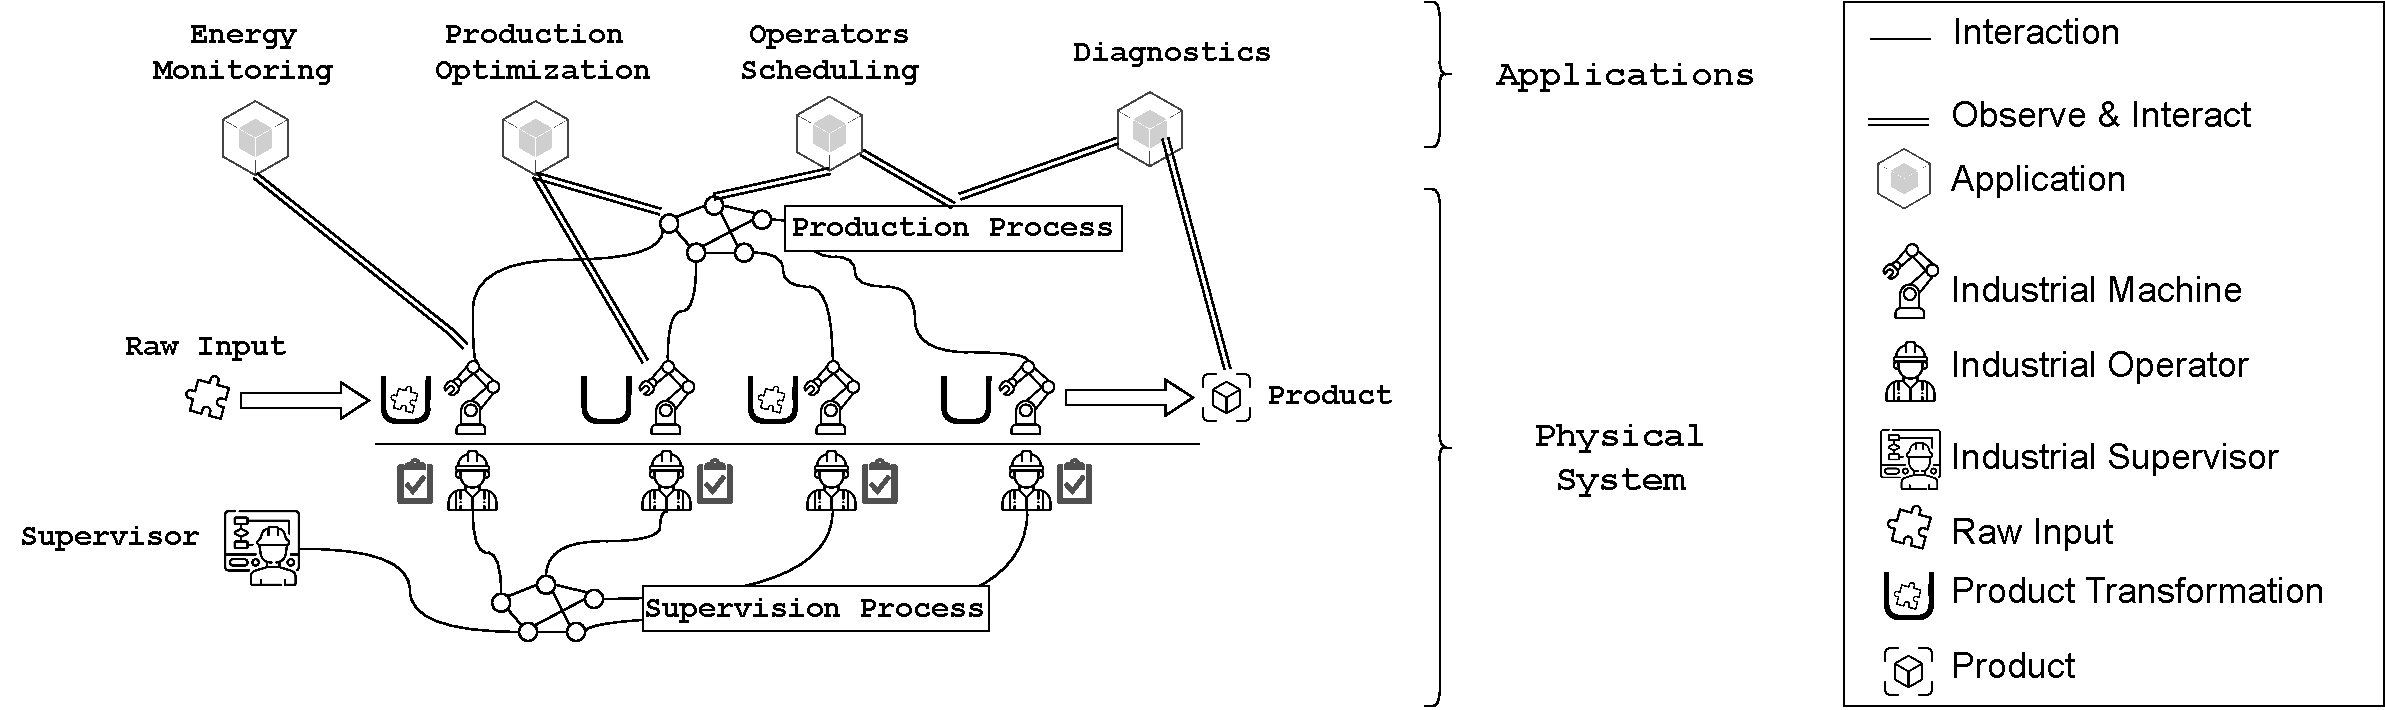
\includegraphics[width=\columnwidth]{figures/dt-mas/smart_manufacturing_scenario.pdf}
    \caption{A reference Smart Manufacturing scenario with multiple physical entities and a set of applications interested in implementing intelligent functionalities on top of the physical deployment.}
    \label{fig:smart_manufacturing_scenario}
\end{figure}

%---------------------------------------------------------------
\subsection{A Smart Manufacturing Scenario}
%---------------------------------------------------------------

A typical production system distributes a diverse array of \textit{machinery}, \textit{operators}, and \textit{processes} throughout the shop-floor environment (as schematically represented in \Cref{fig:smart_manufacturing_scenario}). 
%
These individual components are often organized into \textit{production nodes}, which serve as logical groupings of related machines.
Several nodes make up the overall production plant.

Industrial energy monitoring and optimization is a challenging task, especially in a distributed environment. 
There, such tasks might involve several processes, to selectively turn on different nodes when needed, depending on the external information about the energy cost, while keeping production at an acceptable rate.

As summarized in \Cref{fig:target_functions}, the main target of production and energy optimization is decomposed into three objectives that represent a useful reference to analyse and apply the design principles presented and proposed in this article:
\begin{itemize}
    \item \textbf{Energy Monitoring}: to collect information about the current energy consumption and needs of each production node;
    \item \textbf{Intelligent Coordination}: to dynamically adjust the loads in the production nodes, continuously optimizing the utilisation of resources;
    \item \textbf{Production Optimization}: to make high-level decisions that incorporate data from both individual production nodes and external sources.
\end{itemize}
%
These functionalities are an exemplification of decomposition that can be performed in the design process of an IoT system. In the following, each functionality analyzed towards the definition of components that can implement the IoT system employing either DTs or AAs or a combination of the two.

\begin{figure}
    \centering
    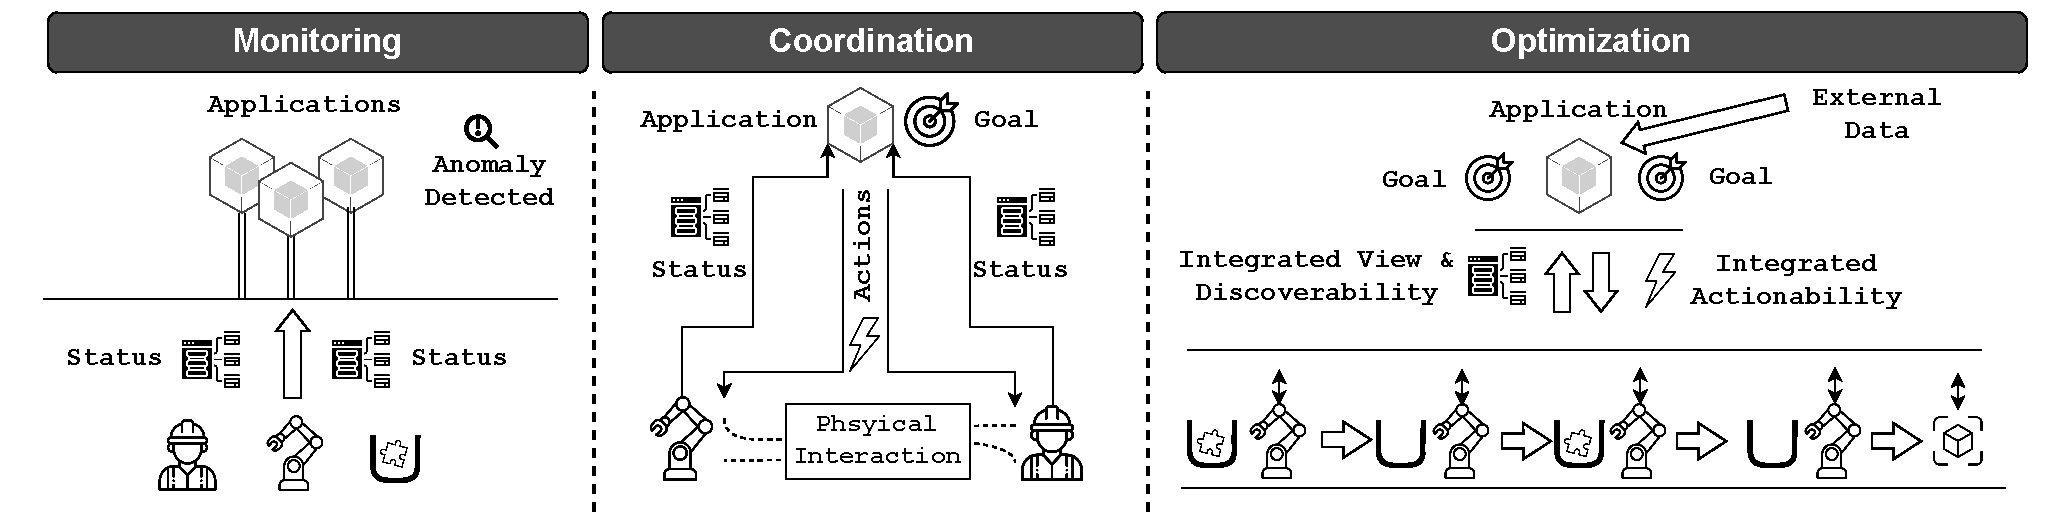
\includegraphics[width=\columnwidth]{figures/dt-mas/target_functions.pdf}
    \caption{Three main objectives that concur to the energy optimization of a Smart Manufacturing plant: Energy Monitoring at the machine level, Intelligent Coordination between robots and operators, and overall Production Optimization based on external factors (e.g. energy cost).}
    \label{fig:target_functions}
\end{figure}

\paragraph{Energy Monitoring}
To make dynamic adjustments to the production process based on the energy consumption of the whole plant it is essential to be able to monitor it in real-time through smart metres embedded in the machines.
Furthermore, it is essential to collect data from each machine or production node to have fine-grained control on what parts of the plant are consuming the most energy.
%
Monitoring can also include some forms of inference to determine whether the observed consumption is considered regular or is an anomaly, and potentially take corrective actions in such cases to improve safety.
%
Finally, prediction or simulation can be used to forecast what the energy consumption is expected to be, given some production tasks, to improve decision-making.

\paragraph{Intelligent Coordination}
This objective involves the use of data collected from the IoT system to introduce coordination capabilities to improve both performance and safety at different levels of deployment (e.g., machine-to-machine or machine-to-operator interactions).
%
For example, machine learning models can be trained to detect patterns and, by continuously monitoring and analyzing data streams from machines and operators, the system can automatically understand the context of the currently performed activities.
%
This is essential to understand the best planning policy to schedule the next tasks as soon as machines or operators are free to perform them.
%
For example, if a portion of the plant is to be shut down for energy saving, the tasks that were queued on those machines should be redistributed across the other active production nodes of the plant.

\paragraph{Production Optimization}
Digital applications can combine real-time data from the physical world and external sources (e.g., market price and production demand) to dynamically optimize manufacturing processes together with all machines, operators, raw materials, and products.
%
This requires decision-making driven by inference of constraints, as well as means to monitor the current situation to adapt according to the real-time state of the system.
%
For this scenario, it is assumed that the market price of energy is provided by an external forecasting system. According to target business rules, the digital layer can optimize production schedules, resource allocation, and task assignment to maximize efficiency and reduce costs.

%---------------------------------------------------------------
\subsection{System Design with AAs and DTs}
\label{ssec:system_design_aas_dts}
%---------------------------------------------------------------


\newcolumntype{P}[1]{>{\centering\arraybackslash}p{#1}}
\newcolumntype{M}[1]{>{\centering\arraybackslash}m{#1}}
\begin{table}
    \centering
    \footnotesize
    \renewcommand{\arraystretch}{1.3}
    \begin{tabularx}{\textwidth}{ p{2cm} | p{2.7cm} p{1.5cm} P{1cm} P{1cm} P{1cm} P{1cm} P{1cm} }
        \hline
        \textbf{Overall Objective} & \textbf{Functionalities} & \textbf{Kind} & \textbf{Specif.} & \textbf{Scoping} & \textbf{Timing} & \textbf{Abst.} & \textbf{$\mu$-arch}\\
        \hline
        \multirow{3}{2cm}{Energy\\Monitoring} 
        & Data collection & n.a. & General & Local & Explicit & DT & \multirow{3}*{E} \\ 

        & \makecell[l]{Anomaly\\Detection} & \makecell[l]{Inference/\\Prediction} & General & Local & Explicit & DT & \\ 

        & \makecell[l]{Corrective\\Reaction} & \makecell[l]{Inference/\\Planning} & Specific & Local & Implicit & Agent & \\
        \hline

        \multirow{3}{2cm}{Intelligent\\Coordination} 
        & \makecell[l]{Activity\\Monitoring} & \makecell[l]{Inference/\\Prediction} & General & Local & Explicit & DT & 
        \multirow{3}*{A}\\ 
        & \makecell[l]{Dynamic\\Planning} & Planning & Specific & Global & Explicit & Agent &\\ 

        & \makecell[l]{Task\\Delegation} & n.a. & General & Local & Implicit & DT &\\ 

        \hline

        \multirow{3}{2cm}{Production\\Optimization} 
        & Decision-making & Inference & Specific & Global & Explicit & Agent & \multirow{3}*{A}\\ 
        & \makecell[l]{Process\\Monitoring} & Inference & General & Global & Explicit & DT & \\ 

        & \makecell[l]{Task\\Delegation} & n.a. & General & Local & Implicit & DT & \\ 
        \hline
    \end{tabularx}
    \caption{Mapping of design principles to the target use case and broad categories of intelligent functionalities (Specif.\ = Specificity, Abst.\ = Abstraction, n.a.\ = not applicable, pure digitalization function).}
    \label{tab:usecase_principles_mapping}
\end{table}


Table \ref{tab:usecase_principles_mapping} reports the mapping between the intelligence functionalities envisioned, the application of the design principles, and the associated micro-architectural design. % following the analysis with respect to the \textit{Specificity}, \textit{Scoping} and \textit{Timing} principles.
%
Each overall objective is decomposed into specific functionalities and associated with the main \textit{ kinds} of intelligent functionalities identified in Section \Cref{ssec:mas+dt:functionalities}.
%
The analysis leads to the adoption of an AA, a DT, or a combination thereof, for functionality, and a different $\mu$-arch for each objective (as shown in \Cref{fig:dt_agents_zoom}), choosing from those presented in \Cref{sec:mas+dt:patterns}

\paragraph{Energy Monitoring}
For this objective, the basic functionality is data collection of a machine's energy consumption.
This functionality has low specificity, since the collected data can be reused for other tasks (e.g., consumption prediction).
Because the data are generated by and associated with a specific PA, the functionality has a local (individual) scope.
An explicit representation of time is required to produce time series.
%
An anomaly detection functionality analyzing time series is also necessary to detect unexpected patterns is expected.
The knowledge for this task remains local to the machine, and results can serve general services (e.g., malfunction notifications).
%
An on-the-fly corrective reaction mechanism is introduced to shut down the machine upon detection of a problem.
This behavior is specific to the monitoring application goal, operates on local data, and can be triggered by events without requiring an explicit time representation.
%
This analysis indicates the need for a machine DT to collect data and detect anomalies, and an AA to implement the emergency shutdown policy.
The resulting micro-architecture corresponds to $\mu$-arch \textbf{(E)} in Figure \ref{fig:architecture}.

\begin{figure}
    \centering
    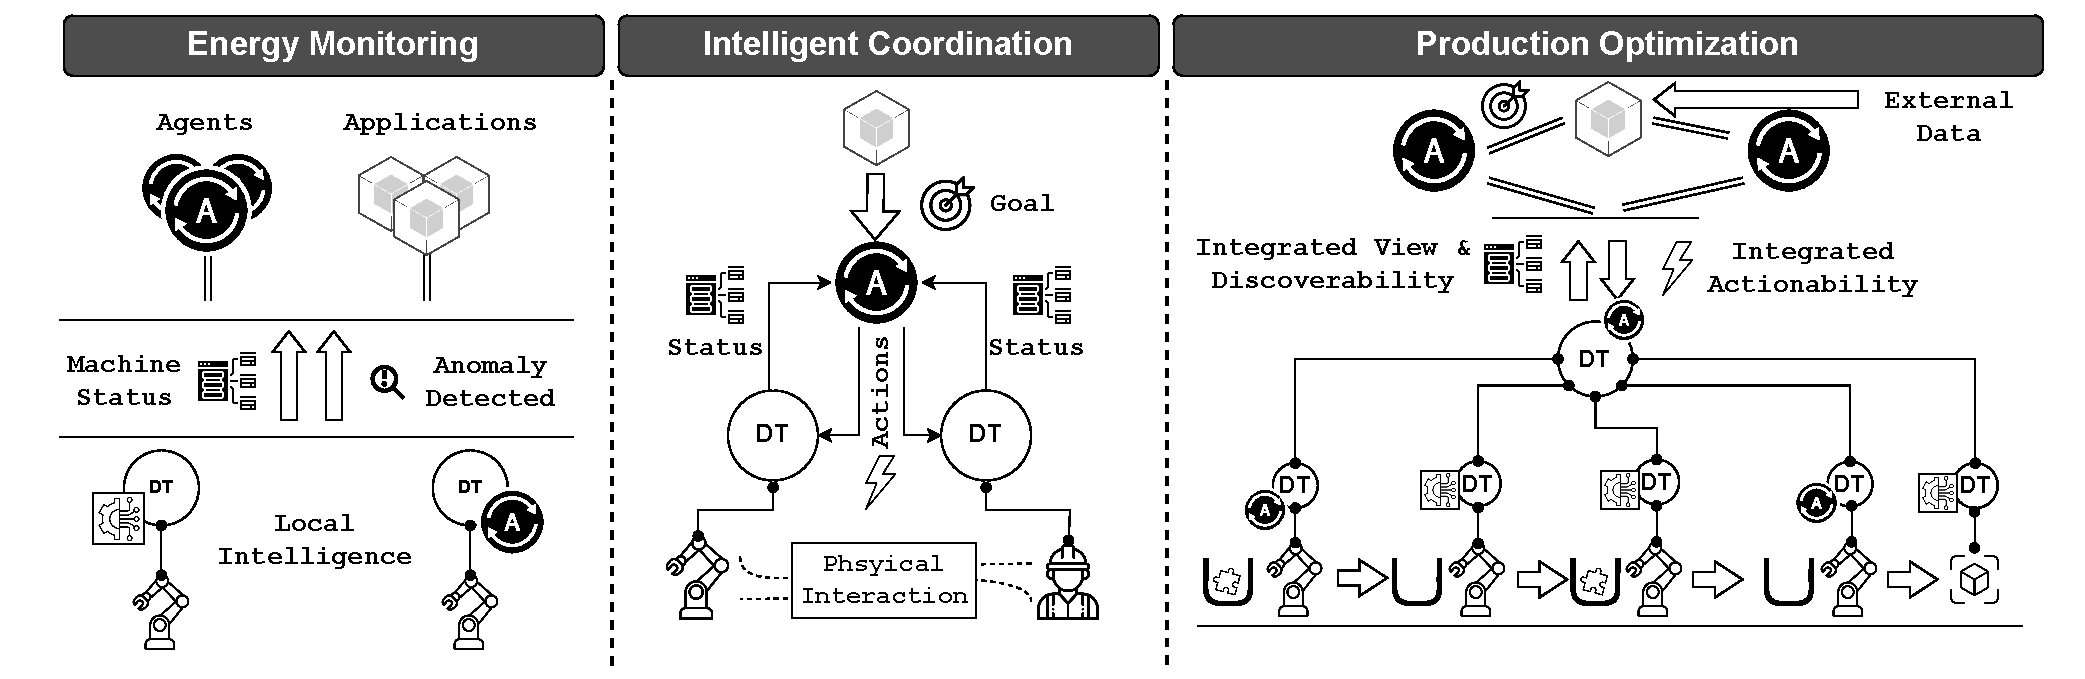
\includegraphics[width=\columnwidth]{figures/dt-mas/dt_agents_zoom.pdf}
    \caption{Three  illustrative instances showcasing the synergistic usage of AAs and DTs as guided by the principles and $\mu$-archs, within the Smart Manufacturing context.}
    \label{fig:dt_agents_zoom}
\end{figure}

\paragraph{Intelligent Coordination}

The data required for this functionality is produced by activity monitoring, which has a local scope on the mirrored PA (e.g., an operator) to infer the current activity and to predict its expected duration; therefore, an explicit representation of time is required.
%
Each machine or operator must also expose a digitalized, personalized interface for receiving delegated tasks.
Task assignment is carried out by a dynamic planning component that operates on aggregated global knowledge obtained from each entity involved in the coordination scenario.

Accordingly, each PA is expected to have a DT that mirrors it and encapsulates activity-monitoring and task-delegation functions tailored to the mirrored entity.
Planning can be implemented by an AA that maintains the global context (for example, of an entire production node) and applies a coordination policy to redirect tasks among machines.
This corresponds to $\mu$-arch \textbf{(A)}, where a single agent consumes multiple DTs as data sources and delegates tasks to each.

\paragraph{Production Optimization}

Optimization at the plant level will be guided by a decision-making functionality based on two sources of data: external data about the market price of electricity for a specific time and date
and data collected locally from the different production nodes. 
%
Depending on the cost of electricity, for instance, the policy may decide to shut down the nodes that are not actively involved in the ongoing process, delegating tasks to different nodes.

Accordingly, $\mu$-arch \textbf{(A)} is the best suited in this scenario, involving a DT that mirrors the production process as the main data source, and an AA enacting the policy and acting on the production nodes.
%
It is worth noting that, having already introduced the DTs of the different production nodes, it is possible to consider linking the DT of the production process to the DTs of the nodes, in a composition pattern that would facilitate the modeling of the production process DT as represented in Figure \ref{fig:dt_agents_zoom}.

%---------------------------------------------------------------
\subsection{Discussion of Resulting Architecture}
%---------------------------------------------------------------

\begin{figure}
    \centering
    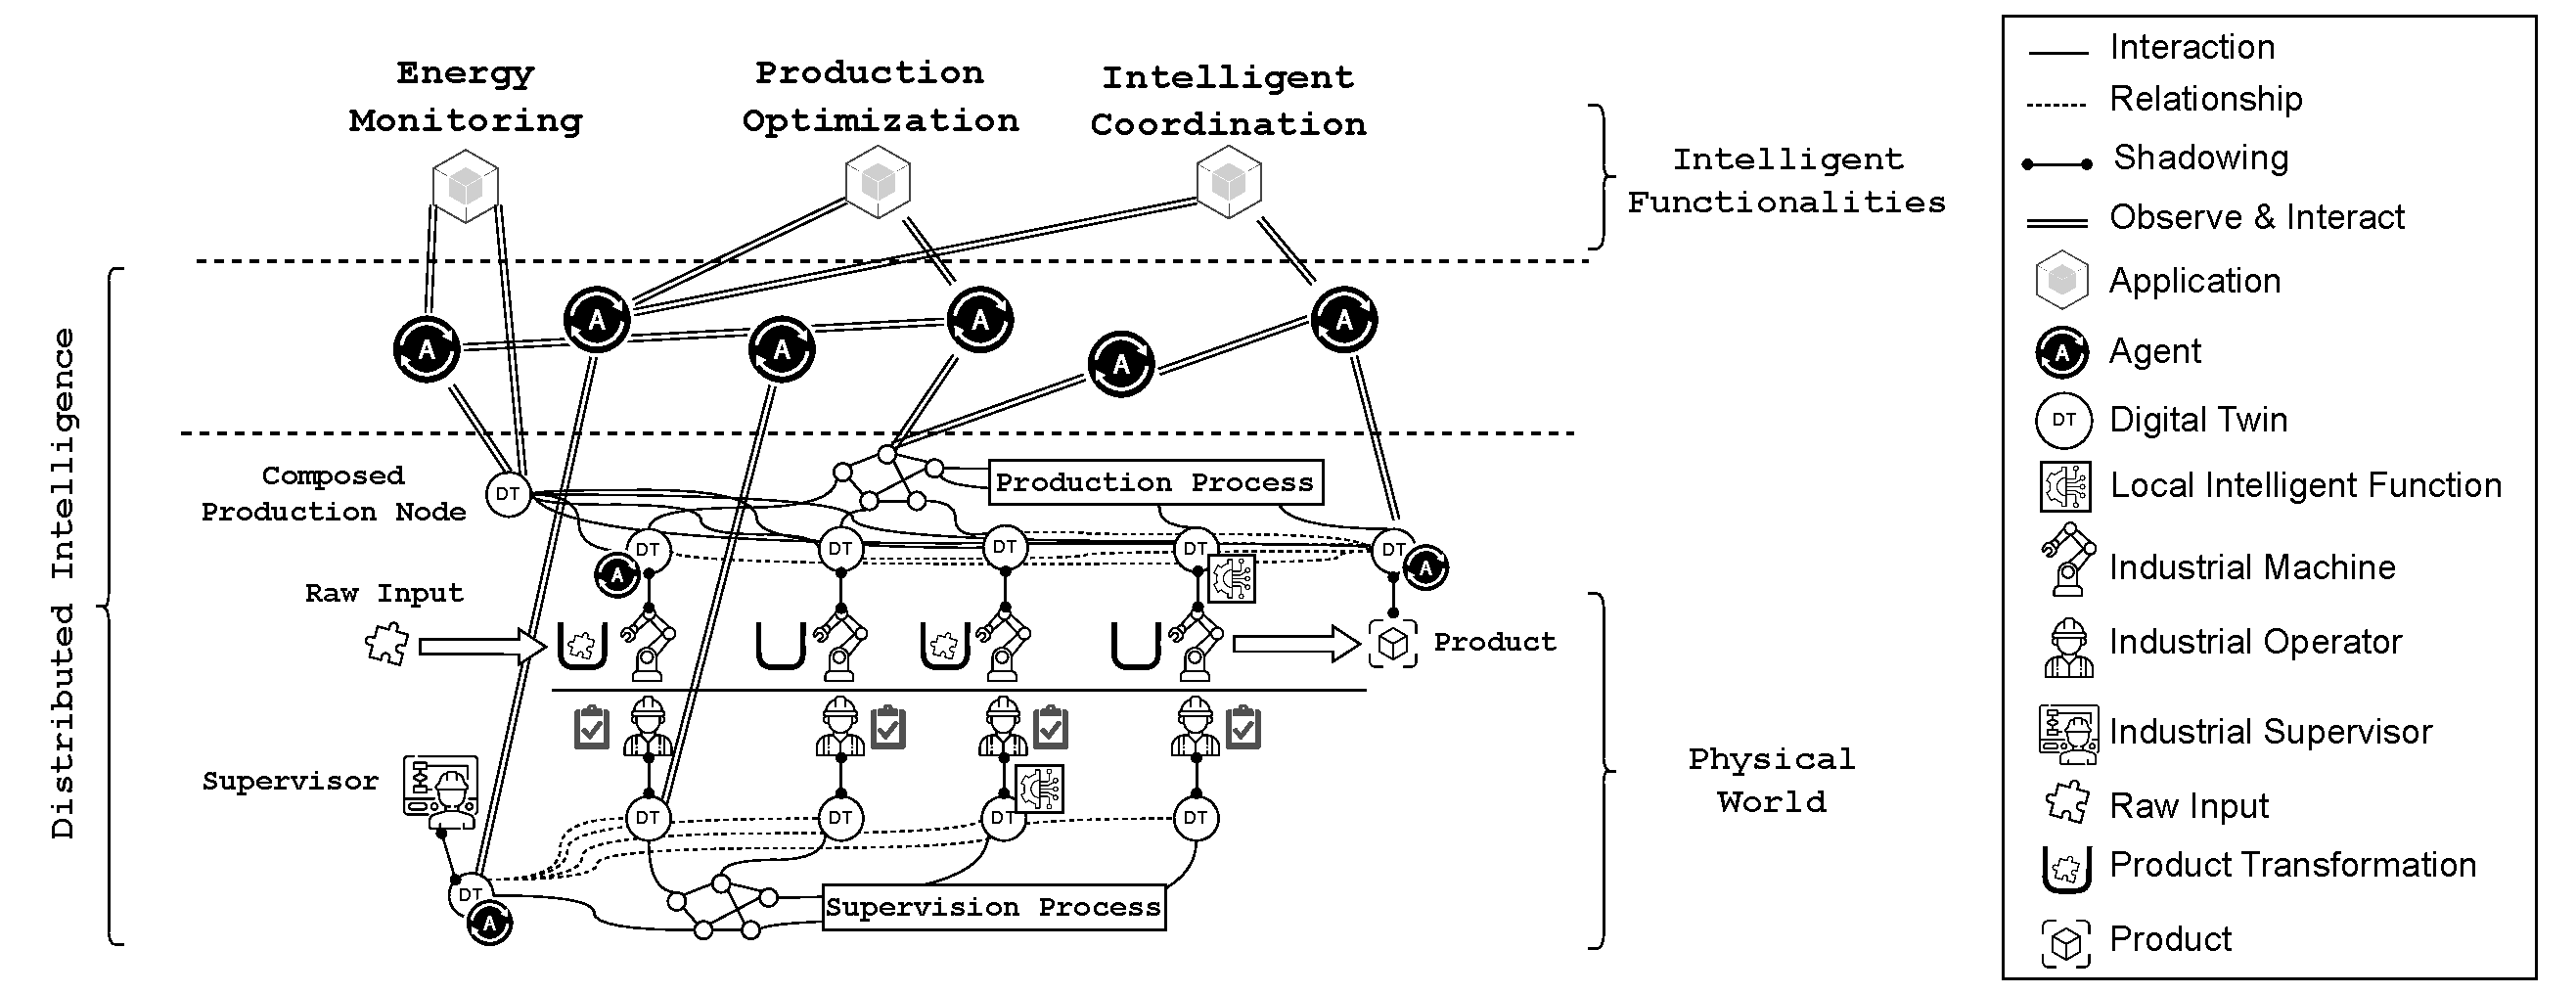
\includegraphics[width=\columnwidth]{figures/dt-mas/dt_agents_smart_manufacturing.pdf}
    \caption{A layered architecture with the combination of DTs and Agents for a Smart Manufacturing reference scenario.}
    \label{fig:dt_agents_smart_manufacturing}
\end{figure}

Figure \ref{fig:dt_agents_smart_manufacturing} schematically illustrates the integrated architecture, using both AAs and DTs, resulting from the application of the proposed design principles and the consequential composition of the identified $\mu$-archs.

The physical world, composed of multiple heterogeneous entities such as machines, operators, raw inputs, and products, can be effectively digitalized through the use of DTs.
These DTs are responsible for representing the associated PAs in cyberspace through interoperable and homogeneous digital replicas, operating locally to the devices and associated just to their context without the need for a global scope.
This approach can also be applied to industrial processes, such as product transformation from raw inputs to final products, the interaction and collaboration between machines and operators, etc.

DTs excel in abstracting and decoupling PAs and processes into modular digital representations, simplifying interaction and integration. They support standardized communication protocols, enhancing interoperability across various platforms and systems, that is critical for integrated manufacturing operations. DTs can be composed of higher-level aggregates, providing a holistic view of the system, which is crucial for understanding interdependencies and optimizing system-wide processes.
%
Moreover, DTs can embed \emph{localized intelligence}, enabling real-time monitoring, anomaly detection, and predictive maintenance, while reducing latency and improving responsiveness.

On the other hand, AAs are designed to operate autonomously, making decisions based on predefined rules or learned behaviors, which allows them to adapt to changing conditions and respond effectively to real-time events. They excel in tasks requiring dynamic coordination and optimization, such as reallocating resources and adjusting schedules based on real-time data and system conditions. Additionally, AAs can be easily scaled and deployed across different parts of the manufacturing system, providing a flexible solution that can grow with the system’s needs.
%
In the envisioned and reference smart manufacturing example, AAs can be distributed across the entire deployment spectrum. They support both local inference and decision-making within a DT, allowing it to achieve its internal target goals, and broader spectrum operations enabling dynamic coordination throughout the production line. This includes adapting planning and task allocation in response to variations in the production line context or external market demand. 

AAs and DTs also benefit significantly from each other. 
AAs benefit from DTs decoupling of complexity when interacting with the physical world and the exploitation of a uniform and interoperable digital representation of it. Conversely, AAs encapsulate decision-making in the system, operating either internally as components of the DT's model (both for single and composed twins), or on a broader scope utilizing the different DTs to collect information and act to improve overall performance and behavior.

An additional benefit of such an integrated approach that combines both DTs and AAs is that the components can evolve separately.
%
Policies can change at the AA level (even online, via learning) without having to modify the DTs. 
Similarly, new and improved DT models could be produced as data is collected about the system, improving support given to the AA decision-making, without changing the AA at all. 

As a final remark, emphasizing modularity, it is worth noting that in this example the decision-making is all performed by AAs. This means that in case of need (e.g.\ some critical failure or an expected contingency), it would be possible to temporarily disable the AAs and let the system fall back to a \emph{manual control}.
Human operators could amend the system as needed, while still benefiting from the real-time data collected by DTs that can continue to operate.

All of these desirable non-functional properties do not come without costs challenges include system integration, resource scaling, and initial deployment complexity, requiring careful planning and optimization strategies to overcome.

%=======================================================
\section{Final Remarks}
%=======================================================

This chapter proposes a practical, software-engineering-oriented view on how to combine \acp{DT} and \ac{MAS} to engineer intelligent \ac{IoT} applications. 
It introduces three design principles (specificity, scoping, timing) to reason about which intelligent functionalities are better encapsulated by DTs or by AAs,
and describes a small catalog of reusable micro-architectures that realize their synergies in practice.

The smart manufacturing example illustrates how the principles drive concrete design choices (e.g., DTs as time-aware, asset-centric providers of data and local services; AAs as goal-driven coordinators for planning and adaptation), and how composed DTs and distributed agents can be combined to achieve modularity, evolvability, and clear separation of concerns. 
Trade-offs and antipatterns are also identified (e.g., avoiding agent-mediated shadowing of PAs), together with opportunities for runtime evolution (independent improvement of DT models or AA policies) and safe fallbacks to manual control.

\paragraph{\ref{rq:4} What are the synergies between \acp{DTE} and \ac{MAS} for the development of intelligent applications?}

DTs and MAS are complementary: DTs supply a time-aware, modelled, and interoperable digital substrate that decouples applications from physical heterogeneity and provides reusable, asset-scoped services (monitoring, prediction, simulation). 
AAs (and MAS) supply goal-oriented, autonomous decision-making, coordination, and adaptation that operate over collections of DTs or on system-level objectives. 
%
Combining them (using the presented principles and micro-architectures) enables clear responsibility separation.
DTs handle data fidelity and temporal modelling, AAs handle planning and policy enactment
while allowing reuse, scalability, and independent evolution of models and policies. 
This synergy supports robust intelligent behaviors (local autonomy, global optimization, online learning) and practical engineering benefits (modularity, interoperability, graceful degradation).


